%電圧レベルの変換
\chapter{論理回路応用}
前章までで、論理回路の基本的な仕組みと作り方について説明した。
本章では、論理回路を実際に使用する際に必要となる応用的な知識について説明する。

\section{オープンコレクタ出力}
今まで、正論理として、論理0を低電位(L)、論理1を高電位(H)として説明してきた。
しかし、オープンコレクタ出力と呼ばれる出力形式では、論理0を低インピーダンス状態、論理1を高インピーダンス状態として扱う。
図\ref{fig:open_collector}の回路図を見てほしい。
\begin{figure}[htbp]
    \begin{minipage}
        {0.45\hsize}
        \centering
        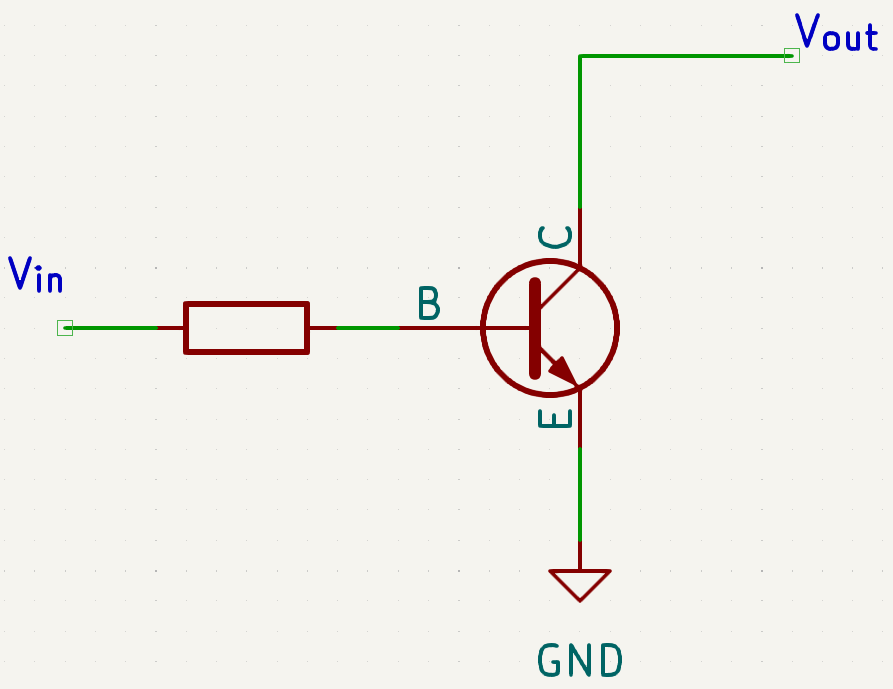
\includegraphics[width=0.8\textwidth]{apply/open_collector.png}
        \caption{出力回路}
        \label{fig:open_collector}
    \end{minipage}
    \begin{minipage}
        {0.45\hsize}
        \centering
        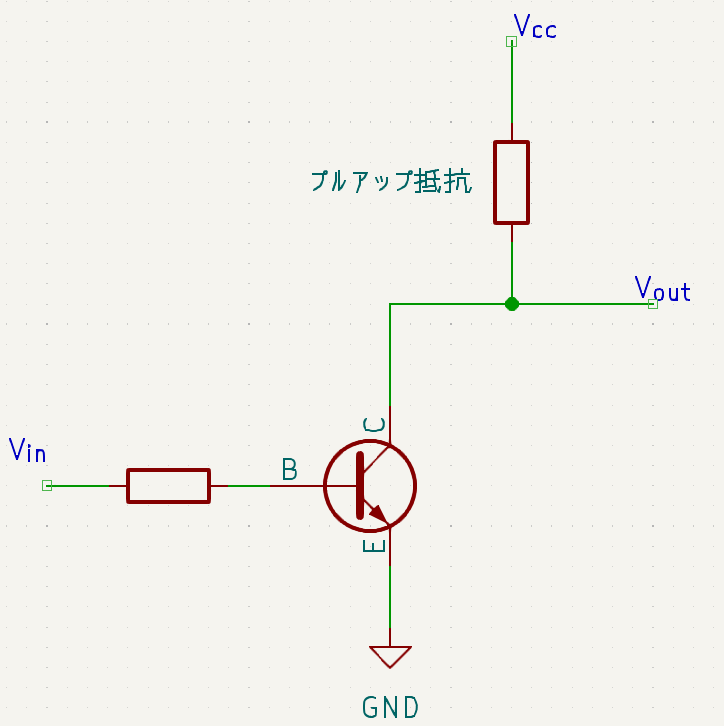
\includegraphics[width=0.8\textwidth]{apply/open_collector_pullup.png}
        \caption{プルアップ抵抗の接続}
        \label{fig:open_collector_pullup}
    \end{minipage}
\end{figure}
この回路は簡単なNOT回路からコレクタに接続されていた抵抗と電源を取り除いたものである。
この回路に$V_{in} = H$を入力すると、トランジスタがオンになるため、トランジスタはとても低い抵抗値とみなせるため、出力$V_{out}$はGNDにとても低い抵抗でつながっている状態となる。
これを低インピーダンス状態と呼ぶ。
一方、$V_{in} = L$を入力すると、トランジスタがオフになるため、トランジスタはとても高い抵抗値とみなせるため、出力$V_{out}$はGNDからとても高い抵抗でつながっている状態となる。
これを高インピーダンス状態と呼ぶ。
このようにオープンコレクタ出力では、論理0を低インピーダンス状態、論理1を高インピーダンス状態として扱う。

オープンコレクタ出力をそのまま扱うことはできないため、プルアップ抵抗と呼ばれる抵抗を出力に接続して使用する。(図\ref{fig:open_collector_pullup}参照)
この回路の動作は、

- $V_{in} = H$の場合、電源→プルアップ抵抗→出力→トランジスタ→GNDの経路ができ、トランジスタが低インピーダンス状態であるため、分圧により出力はGNDに近い低電位となる。(論理0)

- $V_{in} = L$の場合、電源→プルアップ抵抗→出力→トランジスタ→GNDの経路ができるが、トランジスタが高インピーダンス状態であるため、分圧により出力は電源に近い高電位となる。(論理1)

となる。
以上より、プルアップ抵抗とトランジスタの分圧比によって、出力の電圧レベルが決まるため、適切な抵抗値を選択する必要がある。

なおCMOS論理回路の場合、オープンドレイン出力と呼ばれることもあるが、基本的な動作は同じである。

この本ではオープンコレクタ出力を持つ論理回路は回路図上で、出力部に三角形のマークをつけて表記することにする。(図\ref{fig:open_collector_symbol}参照)
\begin{figure}[htbp]
    \centering
    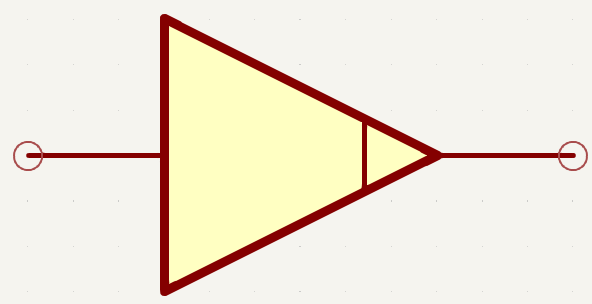
\includegraphics[width=0.2\textwidth]{apply/open_collector_symbol.png}
    \caption{オープンコレクタ出力のバッファ回路の記号}
    \label{fig:open_collector_symbol}
\end{figure}

ここで、オープンコレクタ出力の利点について説明しよう。
通常,各種論理出力をOR演算するときは、OR回路を使用する必要がある。(図\ref{fig:normal_or}参照)
一方で、オープンコレクタ出力の場合、複数の出力をそのまま接続して、プルアップするだけでOR演算が可能である。(図\ref{fig:open_collector_or}参照)
\begin{figure}[htbp]
    \begin{minipage}{0.45\hsize}
        \centering
        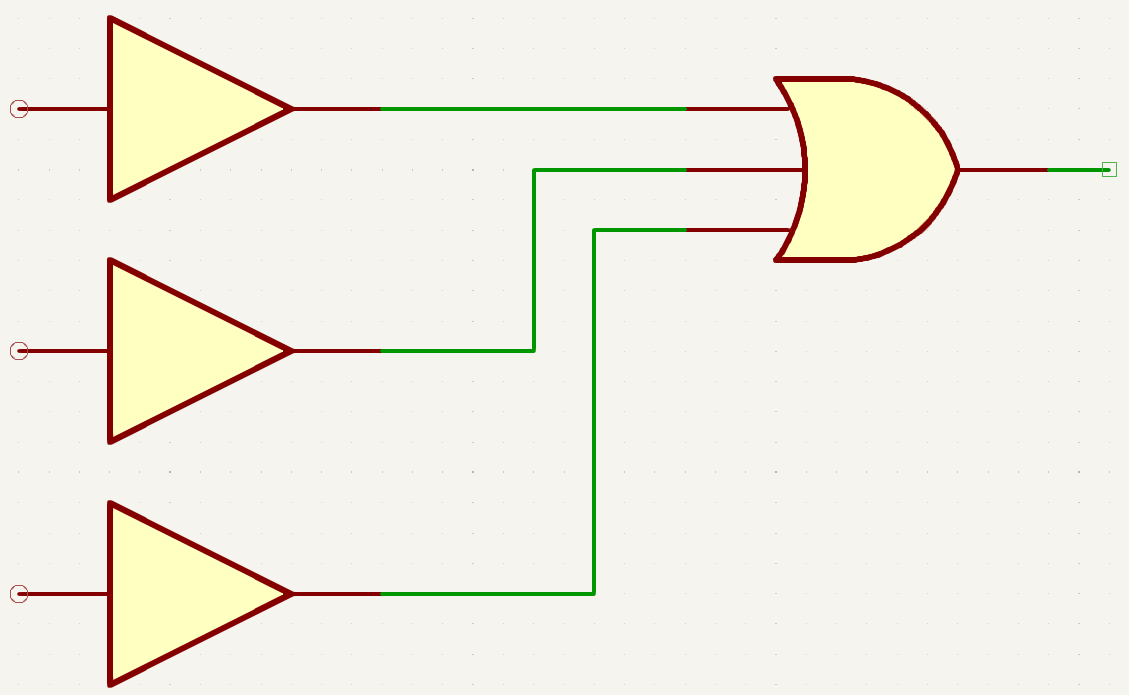
\includegraphics[width=0.6\textwidth]{apply/normal_or.png}
        \caption{通常のOR回路}
        \label{fig:normal_or}
    \end{minipage}
    \begin{minipage}{0.45\hsize}
        \centering
        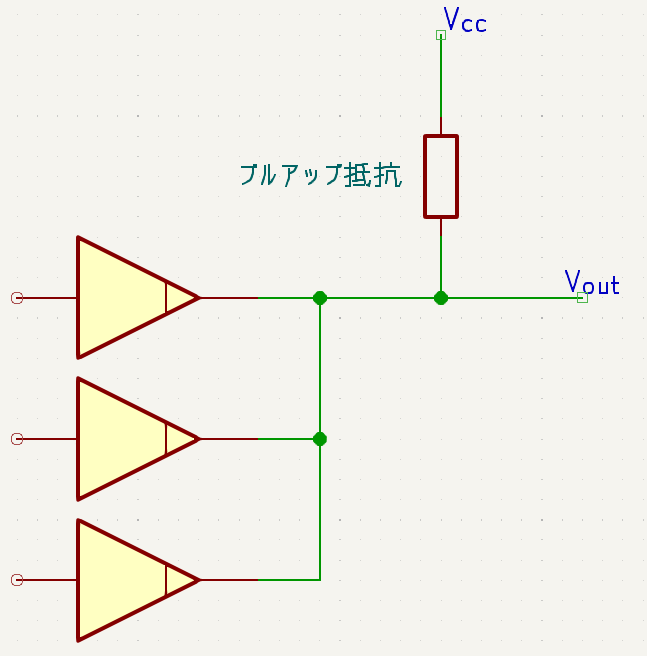
\includegraphics[width=0.6\textwidth]{apply/open_collector_or.png}
        \caption{オープンコレクタ出力によるOR回路}
        \label{fig:open_collector_or}
    \end{minipage}
\end{figure}

図\ref{fig:open_collector_or}の動作を確認しよう。
オープンコレクタ出力すべてが高インピーダンス状態の場合、プルアップ抵抗により出力は高電位(H)となる。
一方で、いずれか1つでも低インピーダンス状態、その部分を電流が通過するため、出力は低電位(L)となる。
このように、オープンコレクタ出力を使用することで、簡単に複数入力OR回路を実現できるという利点がある。これをワイアードORと呼ぶ。
なお負論理の場合は、オープンコレクタ出力を使用してAND回路を実現でき、ワイアードANDと呼ぶ。

このオープンコレクタ出力のTTLのNAND回路の回路図を図\ref{fig:ttl_open_collector_nand}に、オープンドレイン出力のCMOSのNAND回路の回路図を図\ref{fig:cmos_open_collector_nand}に示す。
\begin{figure}[htbp]
    \begin{minipage}{0.65\hsize}
        \centering
        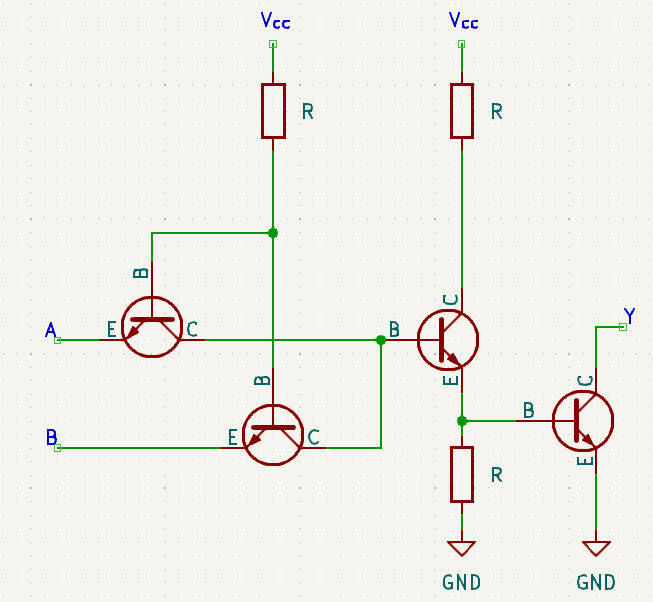
\includegraphics[width=0.8\textwidth]{apply/ttl_open_collector_nand.png}
        \caption{TTLオープンコレクタNAND回路}
        \label{fig:ttl_open_collector_nand}
    \end{minipage}
    \begin{minipage}{0.3\hsize}
        \centering
        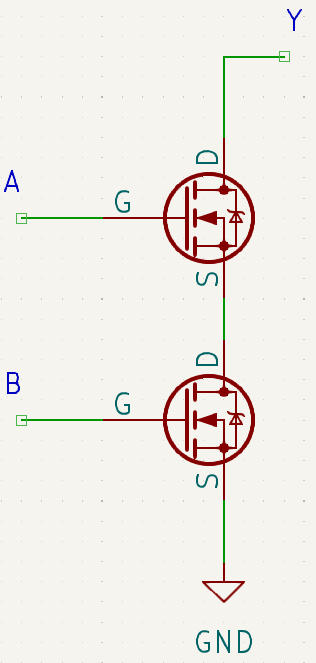
\includegraphics[width=0.8 \textwidth]{apply/cmos_open_collector_nand.png}
        \caption{CMOSオープンドレインNAND回路}
        \label{fig:cmos_open_collector_nand}
    \end{minipage}
\end{figure}

このようにオープンコレクタ出力を実装することができる。
NAND回路以外の論理回路でもオープンコレクタ出力を実装することができる。




\section{各種74シリーズ}
論理回路にはテキサス・インスツルメンツ社が開発した74シリーズと呼ばれるICが広く使われている。74シリーズには様々な種類があり、例えばTTLタイプの場合
\begin{itemize}
    \item 74シリーズ : 標準[standard] 
    \item 74Sシリーズ : 高速型[schottky]
    \item 74LSシリーズ : Sの低消費電力化[low power schottky]
    \item 74ALSシリーズ : LSの改良型[advanced low power schottky]
    \item 74ASシリーズ : Sの高速改良型[advanced schottky]
\end{itemize}
などがある。これらTTLタイプのものはほとんど絶滅しているが、74LSシリーズはまだ存在している。また、CMOSタイプの場合
\begin{itemize}
    \item 74Cシリーズ : CMOS標準[CMOS standard]
    \item 74HCシリーズ : 高速型[high speed CMOS]
    \item 74ACシリーズ : HCの改良型[advanced CMOS]
    \item 74AHCシリーズ : HCのさらなる改良型[advanced high speed CMOS]
    \item 74LVシリーズ : 3.3V以下の電源での動作[low voltage CMOS]
    \item 74LVCシリーズ : LVの高速型[advanced low voltage CMOS]
\end{itemize}
などがある。これらCMOSタイプのものは現在でも広く使われているが、特に74HCシリーズが主流である。

しかし、これらのICはそれぞれ違う電源電圧で動作したり、Hiであると認識する電圧レベルとHiとして出力する電圧レベルが異なったりするため(図\ref{fig:voltage_level})、
異なるシリーズのICを直接接続して使用することはできない。
\begin{figure}[htbp]
    \centering
    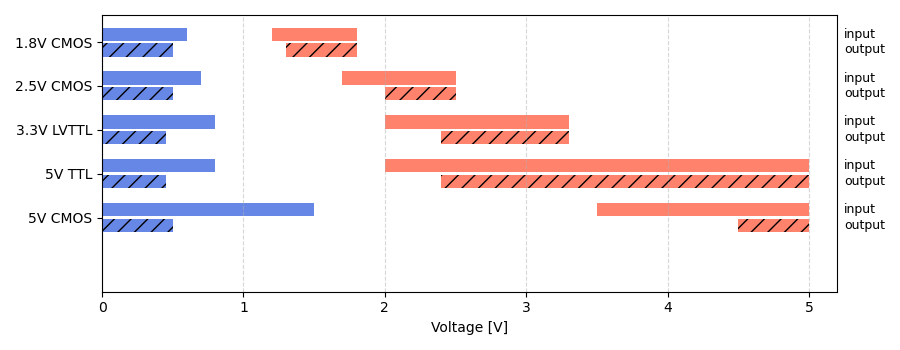
\includegraphics[width=0.95\textwidth]{apply/voltage_level.png}
    \caption{各種74シリーズの電圧レベル}
    \label{fig:voltage_level}
\end{figure}

しかし例外として、入出力トレラントと呼ばれる機能を持つICは、大きな電圧を入力や出力につないだ時でもICが壊れないように設計されているが、
動作は保障されていないので、異なる電圧レベルのIC同士を直接接続して使用するべきではない.

次の部では、異なる電圧レベルのIC同士を接続して使用する方法について説明する。

\section{電圧レベルの変換}

一口に電圧レベルが異なるといっても、出力レベルが入力レベルより高い場合の変換と、出力レベルが入力レベルより低い場合の変換の2種類がある。
まず、出力レベルが入力レベルより高い場合の変換について説明する。
\subsection{出力レベル>入力レベルの場合}
\subsubsection{抵抗分圧}
出力レベル>入力レベルの場合、まず考えることとして、抵抗分圧によって出力レベルを下げる方法がある。(図\ref{fig:voltage_divider}参照)
\begin{figure}[htbp]
    \centering
    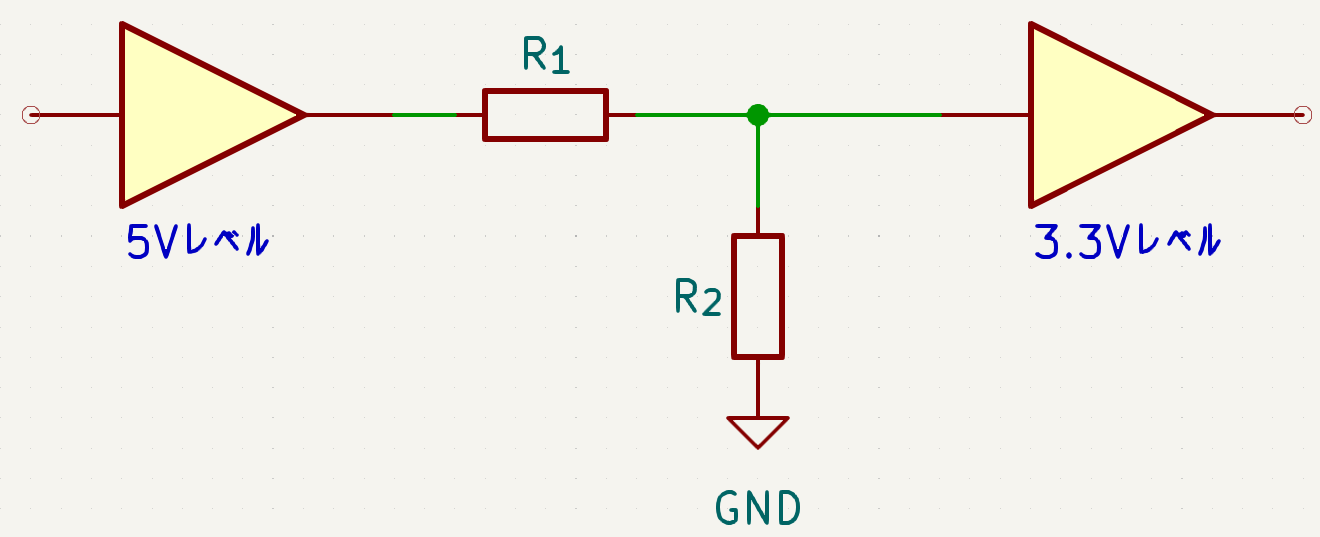
\includegraphics[width=0.5\textwidth]{apply/voltage_divider.png}
    \caption{抵抗分圧による電圧レベル変換}
    \label{fig:voltage_divider}
\end{figure}
この回路では、電圧レベルが5Vの出力を$R_1$と$R_2$の抵抗分圧によって、電圧レベルが3.3Vの入力に接続している。
このとき、
\begin{equation}
    V_{out} = V_{in} \cdot \frac{R_2}{R_1 + R_2}
\end{equation}
となるため、$R_1$と$R_2$の値を適切に選択することで、5Vの出力を3.3Vの入力に接続することができる。
しかし、この方法はゲートの出力がHighのとき、必ず$R_1$と$R_2$に電流が流れるため、消費電力が大きくなるという欠点がある。

また、アマチュアレベルでよく使われている方法として、単純に直列に抵抗を接続する方法がある。(図\ref{fig:series_resistor}参照)
\begin{figure}[htbp]
    \centering
    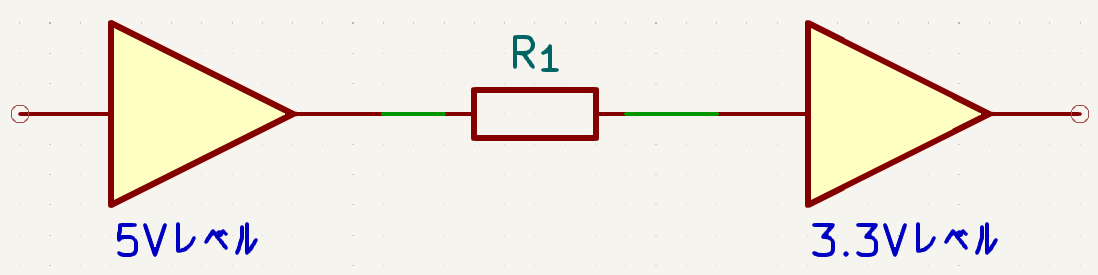
\includegraphics[width=0.5\textwidth]{apply/series_resistor.png}
    \caption{直列抵抗による電圧レベル変換}
    \label{fig:series_resistor}
\end{figure}

この回路は、5Vの出力と3.3Vの入力の間に直列に抵抗を接続している。
この回路は一応動作はするのだが、CMOSの静電気保護用のダイオードに電流が流れ続けるというメーカーの想定外の動作をするため、ICが壊れる可能性がある。(図\ref{fig:esd_diodes}参照)
\begin{figure}[htbp]
    \centering
    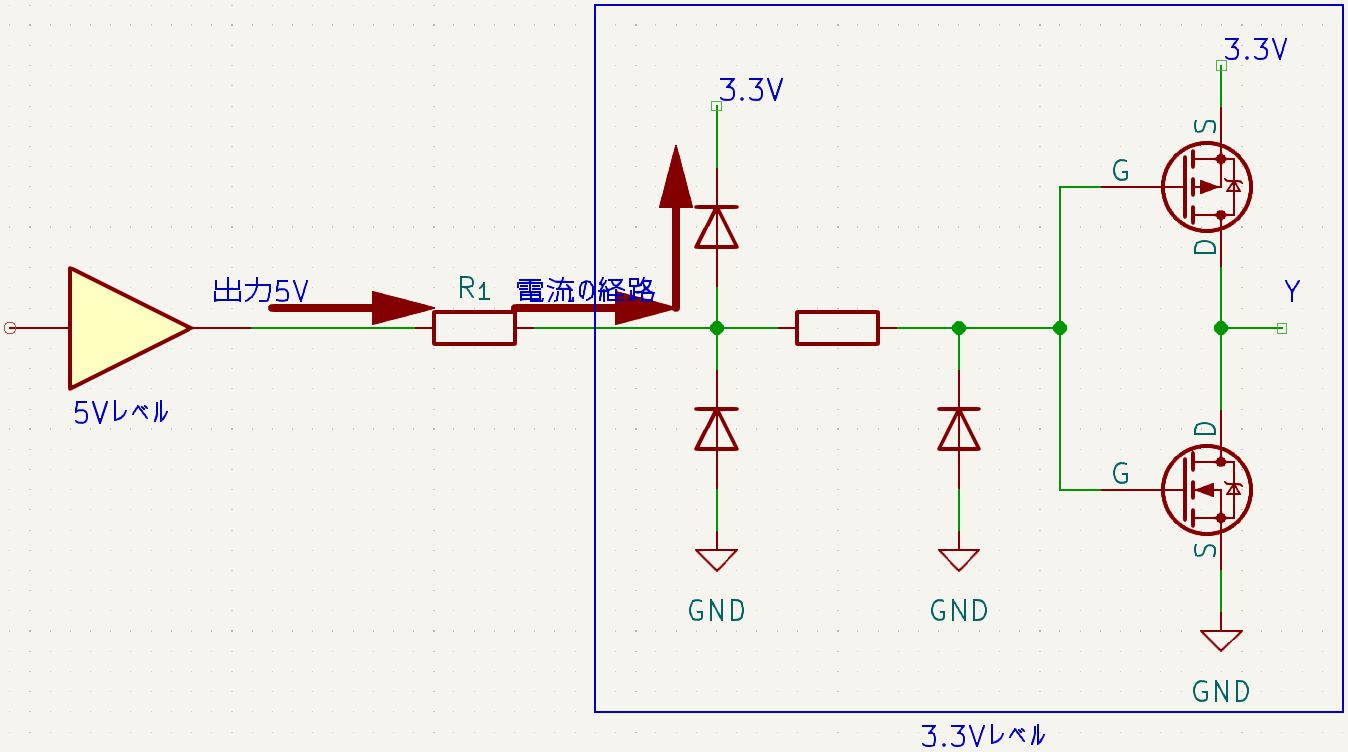
\includegraphics[width=0.5\textwidth]{apply/esd_diodes.png}
    \caption{CMOSの静電気保護用ダイオードに電流が流れ続ける様子}
    \label{fig:esd_diodes}
\end{figure}
そのため、この方法は推奨されない。

\newpage

\subsubsection{オープンコレクタ出力}
もう一つの方法として、オープンコレクタ出力を使用する方法がある。(図\ref{fig:open_collector_level_shift}参照)
\begin{figure}[htbp]
    \centering
    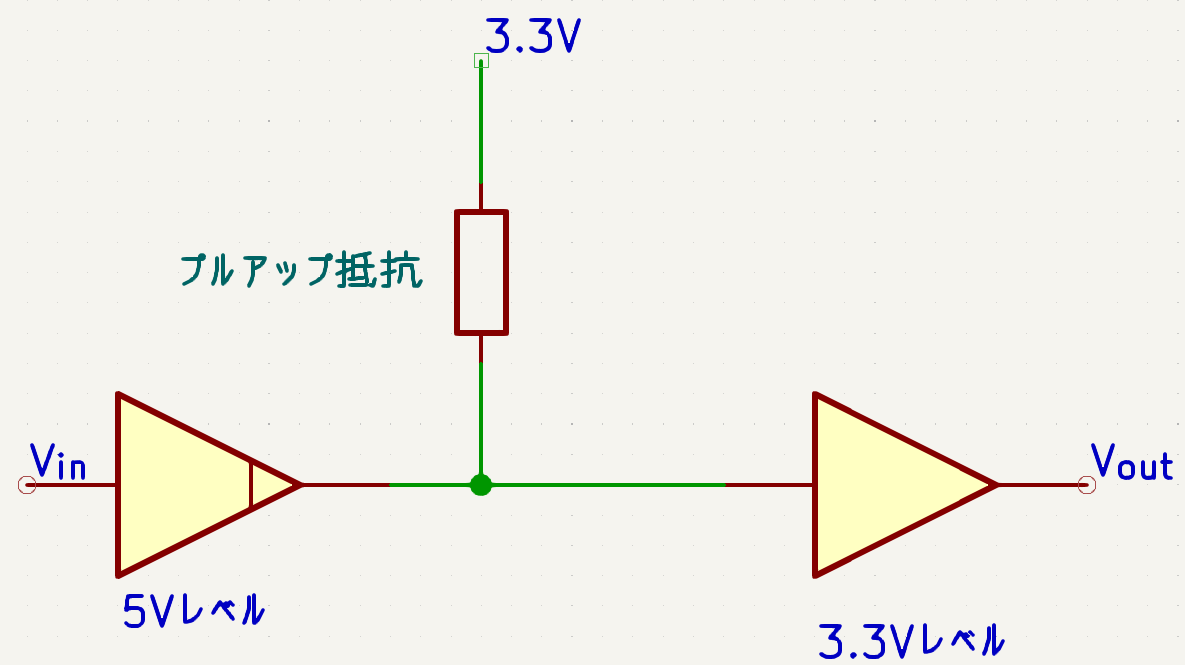
\includegraphics[width=0.5\textwidth]{apply/open_collector_level_shift.png}
    \caption{オープンコレクタ出力による電圧レベル変換}
    \label{fig:open_collector_level_shift}
\end{figure}

論理回路のレベルが5Vであったとしても、オープンコレクタ出力を使用することで、プルアップ抵抗の接続先を3.3Vにすることで、3.3Vの入力に接続することができる。

また、外部にトランジスタを用意することで、5V側がオープンコレクタ出力出なかったとしても、同様の理論でオープンコレクタ出力を実現することもできる。(図\ref{fig:transistor_open_collector}参照)
\begin{figure}[htbp]
    \centering
    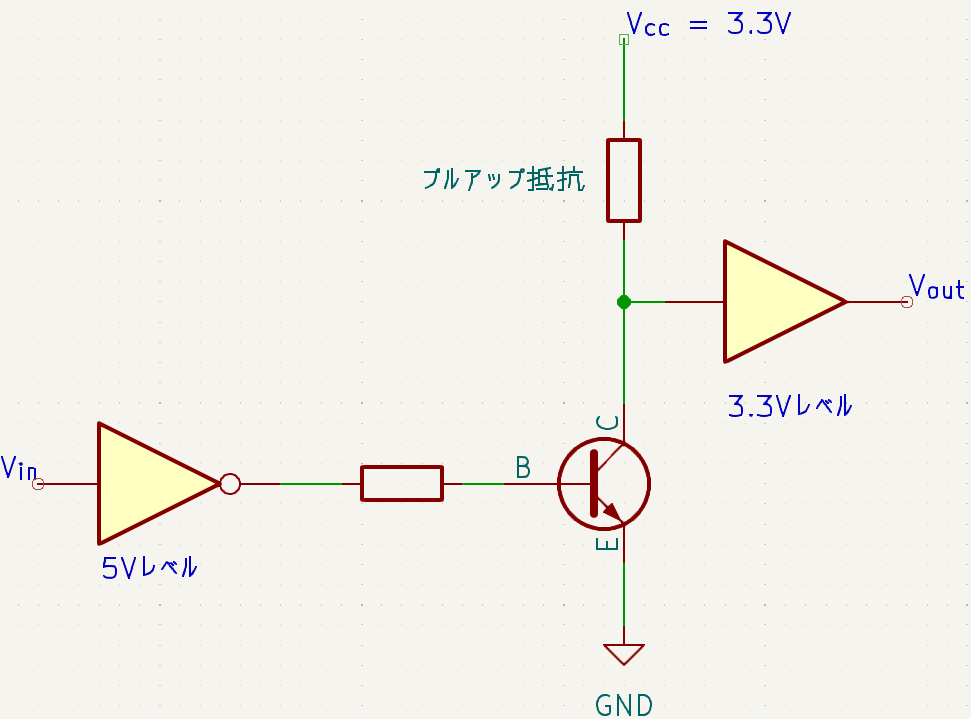
\includegraphics[width=0.5\textwidth]{apply/transistor_open_collector.png}
    \caption{トランジスタを用いたオープンコレクタ出力}
    \label{fig:transistor_open_collector}
\end{figure}

\subsubsection{レベル変換可能なゲートICを使う}
もう一つの方法として、レベル変換可能なゲートICを使用する方法がある。
レベル変換可能なゲートICとは、異なる電圧レベルで動作するデジタル回路間を安全に接続するために設計されたICであり、Texas Instruments社や東芝社などのメーカーから販売されている。
もし迷ったら、この方法を使用することが安全である。

\subsection{出力レベル<入力レベルの場合}
\subsubsection{そのままつなぐ}
出力レベル<入力レベルの場合、ほとんどの場合、そのまま接続しても論理回路が壊れることはない。
ここで、図\ref{fig:voltage_level}を見てほしいのであるが、3.3V LVTTLの出力と5V TTLの入力を接続した場合、
3.3V LVTTLの出力がHighのとき、出力は2.4V以上であるため、5V TTLの入力はHighとして認識する。
このように出力レベル<入力レベルの場合、そのまま接続しても問題ない場合が多い。

一方、3.3V LVTTLの出力と5V CMOSの入力を接続した場合を考えよう。
3.3V LVTTLの出力がHighのとき、出力は2.4V以上であるため、
5V CMOSの入力はHighとして認識する範囲の4.5Vに達しないため、
5V CMOSの入力はHighとして認識しない可能性がある.
この場合は別の方法を使用する必要がある。

\subsubsection{オープンコレクタ出力}
もう一つの方法として、オープンコレクタ出力を使用する方法がある。(図\ref{fig:open_collector_level_shift_low}参照)
\begin{figure}[htbp]
    \centering
    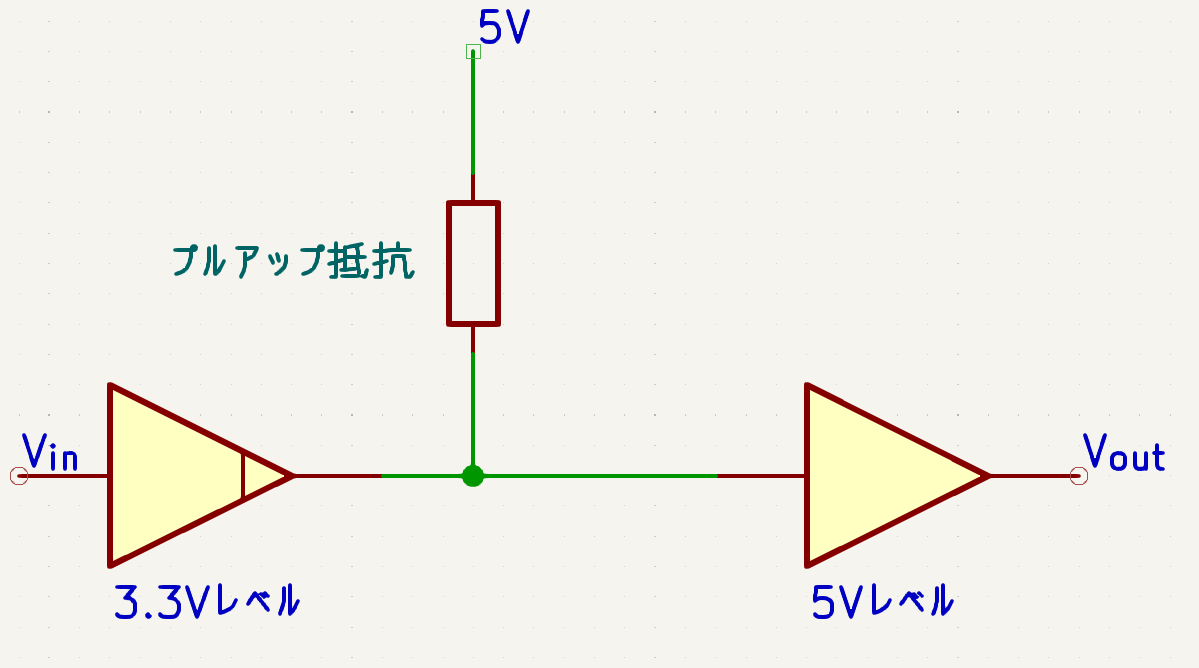
\includegraphics[width=0.5\textwidth]{apply/open_collector_level_shift_low.png}
    \caption{オープンコレクタ出力による電圧レベル変換(低電圧側入力)}
    \label{fig:open_collector_level_shift_low}
\end{figure}
論理回路のレベルが3.3Vであったとしても、オープンコレクタ出力を使用することで、プルアップ抵抗の接続先を5Vにすることで、5Vの入力に接続することができる。
しかし、注意点として、3.3V側の出力端子に5Vの電圧がかかるため、3.3V側のICには出力トレラント機能が必要である。

これもトランジスタを用意することで、5V側がオープンコレクタ出力出なかったとしても、同様の理論でオープンコレクタ出力を実現することもできる。

\subsubsection{レベル変換可能なゲートICを使う}
もう一つの方法として、前の節で紹介した、レベル変換可能なゲートICを使用する方法がある。
やはり、安全性などの観点から、この方法を使用することが推奨される。






